\documentclass{article}
\usepackage{graphicx,palatino-lite,utf8,2112-lecture}

%%%%%%%%%%%%%%%%%%%%%%%%%%%%%%%%%%%%%%%%%%%%%%%%%%%%%%%%%%%%%%%%%%%%%%
\lecture{2}                  %% Lecture number
\title{Encapsulation}
\date{28 August 2012}      %% Date of lecture, e.g., 1 January 2001
%%%%%%%%%%%%%%%%%%%%%%%%%%%%%%%%%%%%%%%%%%%%%%%%%%%%%%%%%%%%%%%%%%%%%%

\begin{document}

\maketitle

\section{The object-oriented programming model}

A major topic of this course is object-oriented design. We use an
object-oriented language, Java, as a vehicle for exploring
object-oriented design. We assume some prior familiarity with Java,
but will focus on how to use it in an object-oriented way.

It is useful to distinguish between object-oriented (OO) _languages_ and
the object-oriented _programming model_. A programming model is an
approach to solving programming problems. There are many programming
models and variants thereof. For example, in addition to the
object-oriented model, there is a _functional_ programming model that
you will learn about in CS 3110. And there are variations on the
object-oriented model such as the _event-driven_ model.

Some languages are designed to support some programming models better
than other, and it makes sense to use an OO language like Java for
learning OO design. But this is not a course about Java. It is a
course about object-oriented design (and other computer science
topics), and the lessons you learn about object-oriented design should
apply to other programming languages.

What makes a language object-oriented? It should support the essential
elements of object-oriented programming. There are three key elements,
which we will discuss in the following three lectures:

\begin{enumerate}
\item Encapsulation
\item Subtyping
\item Inheritance
\end{enumerate}

\section{Encapsulation}

\begin{figure}[b]
\begin{center}
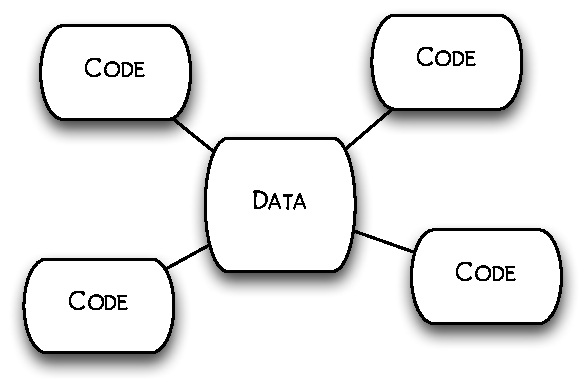
\includegraphics[scale=0.8]{pre-OO}
\end{center}
\caption{Program organization without encapsulation}
\label{pre-OO}
\end{figure}

\begin{figure}
\begin{center}
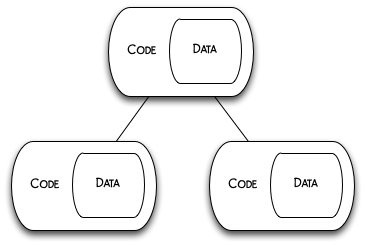
\includegraphics[scale=0.75]{encapsulation}
\end{center}
\caption{Program organization with encapsulation}
\label{encapsulation}
\end{figure}

In early programming languages, the information manipulated by the
program got short shrift. Programs were organized around the
algorithms doing the computation, as illustrated in
Figure~\ref{pre-OO}.  As software systems became
increasingly complex, this model did not work. It did not scale up
to big systems. The problem was that there was no control over
which program code could access a given part of the program. Code
could reach into the program data and use it or update in an arbitrary
way. Reasoning about what programs did was difficult because any
piece of code in the system could affect any other part. A bug in one
software component could corrupt program data and look like a bug in
a different component. Code was hard to maintain and to evolve without
breaking it.

Coordinating access to data is particularly a problem for group
software projects, where programmers are working together. We want to
break the software into distinct _modules_ that can be developed
relatively independently. But in early programming languages it is
difficult to safely share data across different modules.

The idea of encapsulation is to associate data with code and
vice-versa, as suggested by Figure~\ref{encapsulation}. The program
is broken into separate, interacting _modules_ that include both code
and data. Code outside a module cannot directly access the data that
is internal to the module. Any access to a module's data must occur
via its code. Access to the data is _mediated_ by the code, and
changes to the way information is represented tend less to propagate
to other modules.

\section{An example: rational numbers}

In an object-oriented language like Java, encapsulation is provided by
classes. The class and its code are shared by all objects of that
class (the _instances_ of the class), and the class's code can mediate
access to all information stored in instances. For example, consider
the class implementing rational numbers, shown in
Figure~\ref{rational-code}.

\begin{figure}
\begin{code}
\small
class Rational \{ // a rational number p/q where p is numerator and d is the denominator
  private int p,q
    // invariant: q > 0, gcd(p,q) = 1
\hbox{}
  /** Update this to be this+r. */
  public void add(Rational r) \{
    int g = gcd(q, r.q);
    p = r.q/g * p + q/g * r.p;
  \}
\hbox{}
  /** Create num/den. Requires den != 0. */
  public Rational (int num, int den) \{
    if (den < 0) \{
      num = -num;
      den = -den;
    \}
    int g = gcd(num,den);
    p = num/g;
    q = den/g;
  \}

  public boolean equals(Rational r) \{
    return (p == r.p && q = r.q);
  \}

  /** Returns x+y. */
  public static Rational plus(Rational x, Rational y) \{
    Rational z = new Rational(x.p, x.q);
    z.add(y);
    return z;
  \}
\}
\end{code}
\caption{Example: Rational numbers}
\label{rational-code}
\end{figure}

There are many things to note about this implementation. The data in
"Rational" objects is the fields "p" and "q", which are marked
"private" to indicate that they should be encapsulated inside the
class. The keywords "public" and "private" are known as _visibility
modifiers_, because they control which parts of the class are visible
outside the class, and hence can be accessed.

The methods "add" and "equals" and the constructor "Rational" are marked "public"
and hence can be used by external clients. External client code might
look like this:

\begin{code}
Rational r1 = new Rational(1,2);
r1.add(new Rational(2,3));
// r1 now equals 5/6
\end{code}

Inside the method "add", there is a special variable "this" that
refers to the object on which the method was invoked, called the
_receiver object_. It happens that "add" does not mention "this"
explicitly, but it does refer to the fields of "this" as "p" and "q".
Writing these names is equivalent to writing "this.p" and "this.q"
respectively.

The method "plus" is a _static_ method, which means that it does not
have a receiver object. The special variable "this" is not _in scope_
in a static method. That means it cannot be named within the method. A
static method should be called using the name of its class, as in the
following code:

\begin{code}
Rational r3 = Rational.plus(r1, r2);
\end{code}

\noindent It is also possible to declare fields to be static, in which
case they are shared by all objects of their class. However, this
practice should usually be avoided, and even static methods
(except for constructors) should be used sparingly because they limit
reuse and extensibility of the code.

An early comment expresses an _invariant_ regarding the fields "p" and
"q".  An invariant is something that is always true\footnote{Sometimes
invariants can be violated temporarily.} It says "q" is always
positive and that the rational number is always stored in reduced form
where "p" and "q" are relatively prime. Because the fields "p" and "q"
are private, the code of the class can enforce this invariant. Code
outside the current class has no way to, say, modify "q" to be zero,
which is helpful because methods of the class can ignore the
possiblity of a zero denominator.

The class constructor, named "Rational", is also static in the sense
that it is not called using a receiver object. However, the variable
"this" and its fields _are_ in scope inside the constructor. They
refer to the object currently being constructed. Notice that the
constructor does not simply accept the numerator and denominator
directly, but instead computes a new numerator and denominator that
represent the same number while satisfying the invariant.

Because of the invariant, the method "equals" can be implemented very
simply and efficiently, by comparing the corresponding fields of
"this" and "r". This works because the invariant ensures there is only
one way to represent a given rational number. Without the invariant,
we would have to write something more expensive like the following:

\begin{code}
  public boolean equals(Rational r) \{
    return (p*r.q == q*r.p);
  \}
\end{code}

\section{Names and packages}

The dot symbol "." is used for several things in Java. It is used to
indicate use of a method or field. Beyond this, it is used to indicate
which package a class lives in. In an expression like
"cs2112.lec02.Rational.plus", the first part ("cs2112.lec02") is the
name of a _package_ in which the Rational class is located. Package
names can have dots inside them, and those happen to define how Java
source code and compiled code are stored onto the file system.
However, it is incorrect to think of "cs2112.lec02" as being
``inside'' "cs2112". In particular, something that is made visible
just to classes in the "cs2112" package will not be visible to classes
in the "cs2112.lec02" package.

\section{The main method}

A Java program is simply a class with a static "main" method. It must
have the following signature:

\begin{code}
public static void main(String[] args);
\end{code}

Because it is static, "main" can be called when no object of its class is
available. Extra arguments supplied to the program by the operating
system are made available in the array "args".

\section{Objects vs. primitive values, and autoboxing}

_These notes are still under construction_

\end{document}
